\section{Experimental Results}\label{sec:results}
In order to evaluate our method, we perform artifact correction and classification through the pipeline illustrated in \cref{fig:ProgramPipeline} on the BCI Competition IV dataset 2a \citep{brunner2008bci}. The dataset contains 4-class motor imagery EEG data from 9 subjects. Each subject participated in two sessions of 6 runs on different days. The training data is from the first session, and the test data is from the second. A run consist of 48 labeled trials, divided evenly between the 4 classes. Each trial measured the brain signals of a subject on 22 EEG channels and 3 EOG channels. We disregard the EOG channels since we are interested in correcting artifacts without any reference signals. Examples of trials, channels, runs, and sessions are shown in \cref{fig:dataset}. What we refer to as a trial is a three second span (750 samples) of motor imagery, without the cue, break, etc. in between.

\begin{figure*}
	\centering
	\begin{adjustbox}{width=\textwidth}
		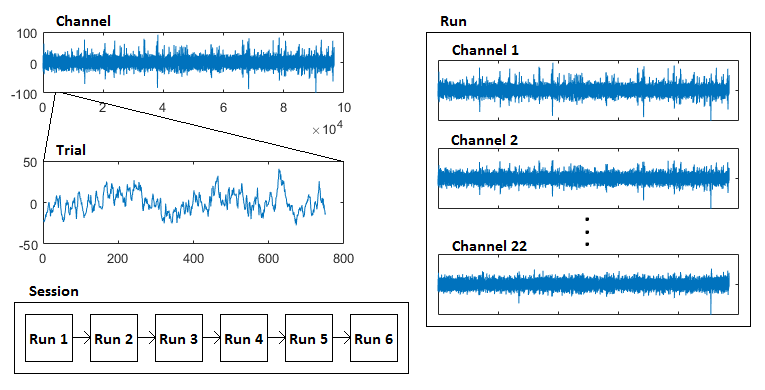
\includegraphics{figures/bciiv2a.png}
	\end{adjustbox}
	\caption{Sessions, runs, channels, trials, and the relations between them.}
	\label{fig:dataset}
\end{figure*}

We set up two pipelines to be compared. The first consists of artifact correction, followed by feature extraction with FBCSP and Random Forest classification. The second pipeline is identical but without the artifact correction step, which leaves us with FBCSP and Random Forest. We run Random Forest with six predefined seeds and return the mean to ensure reproducibility.
To test the generality of the pipeline, we perform 6-fold cross-validation on the training data using five runs for training and one for validation. We run 200 iterations of Bayesian Optimization to select hyperparameters for each pipeline. The best hyperparameters from cross-validation for each pipeline is then used to construct the pipeline for the final evaluation, where we predict the labels for the evaluation data. We repeat this for each subject. 
\cref{fig:results} shows the obtained accuracies with(C2) and without (C1) artifact correction for each subject.

\begin{table}[H]
	\begin{tabular}{@{}l|llll@{}} \toprule
		S					  & C1             & C2             & C3             & C4             \\ \midrule
		1                     & 83,04          & 82,29          & 81,42          & \textbf{83,85} \\
		2                     & 57,18          & \textbf{57,29} & \textbf{57,29} & 54,67 		  \\
		3                     & 78,18          & \textbf{79,16} & \textbf{79,16} & 75,64          \\
		4                     & 65,74          & 63,83          & 65,05          & \textbf{67,71} \\
		5                     & \textbf{58,85} & 55,21          & 55,21          & 56,94          \\
		6                     & \textbf{50,23} & 45,72          & 48,03          & 48,18          \\
		7                     & \textbf{68,75} & 68,69          & 68,69          & 67,94          \\
		8                     & 74,54          & 74,54          & \textbf{74,65} & 74,48          \\
		9                     & \textbf{75,64} & 72,97          & 72,80          & 75,52 		  \\ \bottomrule
	\end{tabular}
	\centering
	\caption{Accuracies for the best runs using 4 different setups. The best results are marked with bold. C1 is the baseline testing without OACL, C2 is 200 iterations of BO with OACL, C3 is 300 iterations of BO with OACL, C4 is 200 iterations with fixed parameters}
	\label{fig:results}
\end{table}

With 200 iterations the artifact correction did not overall yield better results than with no artifact correction and, in fact performed worse on some subjects. One possible cause may be that optimizing 27 parameters over 200 iterations is not a large enough budget to find optimal values for all hyperparameters, since the search space for 27 parameters is much larger than the search space for the 2 parameters optimized in the pipeline with no artifact correction. For this reason, we increased the iterations from 200 to 300 to see if this would yield improved results as illustrated in \cref{fig:results}. As can be seen, the accuracy increased for three subjects, decreased for two, and remained the same for four. This indicates that 300 iterations are still not enough to optimize over such a large search space.

Because our objective is to determine whether removing the artifact signal from the raw signal yields improvements in classification accuracy, we manually set the non-artifact correction parameters to the best obtained values found in the non-correction evaluations, instead of further increasing the number of iterations. This introduces the assumption that good parameters without OACL are also good with OACL. Therefore, we now optimize the $\theta$ parameters to find the values that yield the highest accuracy. The results of running 200 iterations with this assumption are shown in \cref{fig:results}, as C4. The results improved for two subjects, and worsened for the remaining seven, when compared to C1. Once again we were not able to improvement upon the results obtained in C1. This configuration may also need more iterations since the search space is almost the same as in C2 and C3.

\subsection{Discussion}\label{sec:discussion}
% OACL ranges, may not only remove Ocular artifacts.
In the original OACL paper by \citep{li2015ocular}, the relative height ranges specified in \cref{eq:ranges} were determined by manual inspection of the characteristics of ocular artifacts. Since we generalized this as an optimization of hyperparameters, the found ranges are no longer guaranteed to be optimal in regards to ocular artifacts, but instead optimized for correcting the artifacts that most negatively affects the classification results. In fact, since we optimize the ranges for maximal classification accuracy, the method may be removing parts of the signal that are technically not artifacts, but removing them increases the performance of the classification model.

% Optimizing BO settings, and changing the kernel
Moreover, we have run Bayesian optimization with the default settings with regards to exploration vs. exploitation. Since running experiments on the pipeline with OACL is relatively expensive, it would be better to tune BO to spend more time on selecting the best candidate future sample to perform the next experiment on. The most used kernel for optimization problems used with BO is the squared exponential, this is however not always a good kernel, since sampling from a GP with this kernel, often will result in a unrealistic smooth function. Therefore we use Matérn 5/2 which is proposed in \citep{snoek2012practical}. Although this kernel function will be less smooth than the standard squared exponential, it might not be a suitable candidate for out optimization problem. In fact, BO might not even be possible with the domain of our parameters. BO assumes that input parameters with values close to each other, will have relatively similar outputs. Since our input space contains variables from many different algorithms, including FB, CSP and OACL, this assumption might however not hold. 

% Removing residual artifacts
As explained in \cite{hoffmann2008correction}, residual artifacts were still present after noise reduction methods were applied. We have also observed that residual artifacts are present, this can be seen in \cref{fig:oacl-signals}, where an event is registered around $x \approx 170$, but the following desynchronization/synchronization is not registered. A way that this could be handled is to always check if a residual artifact is present when an artifact is registered that, and mark it. These signals might need a separate $\theta$, since the signature of these artifacts is quite different from the artifacts introduced by eye blinks.

Since OACL is not restricted to finding ocular artifacts, a generalization of theta values for each channel, might not be optimal. This is due to the difference in how various artifacts shows in EEG data. A better way, might be to construct a classifier for artifacts, and use a different theta value for each such artifact. The classifier will then be used in the cleaning of new EEG signals, to remove just the right amount of artifact signal, based on the type of artifact. Furthermore, theta values are found based on optimization through BO. An alternative would be optimization through logistic regression. 
Since OACL is not restricted to finding ocular artifacts, a generalization of theta values for each channel, might not be optimal. This is due to the difference in how various artifacts shows in EEG data. A better way, might be to construct a classifier for artifacts, and use a different theta value for each such artifact. The classifier will then be used in the cleaning of new EEG signals, to remove just the right amount of artifact signal, based on the type of artifact. 

Furthermore, theta values are found based on optimization through BO. An alternative would be optimization through logistic regression as proposed in the original OACL method by \citet{li2015ocular}. Even though their technique considered only binary classification, it would be possible to expand their logistic regression approach to the multi-class case, by applying an one-vs-rest algorithm to construct 4-binary classifiers. This should reduce the Bayesian optimization search space, and increase the results of applying the ocular artifact correction.

% Using more oacl ranges
In this study we used just one range for OACL, but the method can easily be extended to use and optimize multiple ranges. That would likely increase the accuracy further, since different artifacts show up in different ranges. Each range adds to the dimensionality of the search space. Alternatively, a wavelet transform approach could be used for the removal step \citep{krishnaveni2006automatic}.

% More clever use of filter bank
The filter bank can be improved by optimizing over a wider variety of sub-bands, for example by mixing sub-bands with differing spans such as [4-8] and [8-11]. This would increase the complexity of the input space., which in turn would make the optimization of all parameters harder. 